\chapter{Objectives and Methodology}

\section{Objectives}

Keeping all of this in mind, we can now bring up the main purpose of this investigation labor, which is to generate a behavioral focused on tracking and actively following a person, making use of a robot. This internal process of transformation of the stimuli into a movement will be accomplished using \textbf{convolutional neural networks}.\\

With all this in mind, the objective of the present work has been to get a little further on \textbf{deep learning applied to robotics}, developing two consecutive components, each one functionally focused on a purpose. They will be introduced right below.
	\begin{itemize}
		\item \textit{Detection:} As it will be described on the suitable chapter, we will build a component (\texttt{Object Detector}) which implements \textbf{a generic object detection algorithm} on an incoming video stream. This component will be ready to work in \emph{real time}.
		
		As it can be inferred, it will not provide a response \textit{per se}. Its visible output will be to draw \emph{bounding boxes} surrounding each detected object, indicating as well the class where that particular object belongs (person, airplane, dog, etc.), and its score (confidence in \%).
		
		\item \textit{Tracking and following:} As we want to implement a following behavioral, our main objective here is to \textbf{identify and track} the person to follow, which will semantically be called \emph{mom}. The component that comprehends the previous detection behavioral and this new one will be named \texttt{Follow Person}. The great advantage here is the strength a CNN can achieve under variable light conditions. That makes this technique perfectly suitable to command physical actuators on a robot.
		
		We will make use of the detected people (with the technique followed on the previously described node and constraining the result to only retain people detection), and look for the face of each one of them. Later, we will make use of another neural network technique, called a \emph{siamese network} (it will be properly explained later) to identify them. It will allow us to find \emph{mom}, in case it is being seen by the camera, and command a proper response to the robot with the objective of following \emph{mom}.
	\end{itemize}

As we have said before, these two nodes/components are successive. Thus, they will share an important part of the global objectives.\\

We will start breaking down the common objectives between both applications, into three functional blocks:

\begin{itemize}
	\item \textit{Design:} both milestones have been preceded by a first \textbf{documentation} phase. While the theoretical base was learned and achieved, some papers and examples were investigated. We will go some deeper in each section.
	
	Later, a more specific design phase will be to specify the structure of the nodes.
	From now on, we will have to perform several tasks simultaneously:
	\begin{itemize}
		\item Grabbing the incoming image(s) from the sensor(s).
		\item Processing the image(s).
		\item Properly update the GUI (\textit{Graphical User Interface}) with the image(s) and the outputs of the processing.
		\item \textit{Only on the following node:} send the computed response order to the actuators.
	\end{itemize}
	%
	These tasks should follow an \emph{asynchronous schema} every time, to avoid blocks between tasks, and taking advantage of some shared memory to exchange inputs/outputs. Besides, this allows us to have a custom iteration period for each task: we shouldn't have to wait until the neural network finishes feed-forwarding the image to refresh the \emph{GUI}. On a high level structure, it could follow the schema on the \autoref{fig:2_tasks}.
	
	\begin{figure}[h]
		\centering
		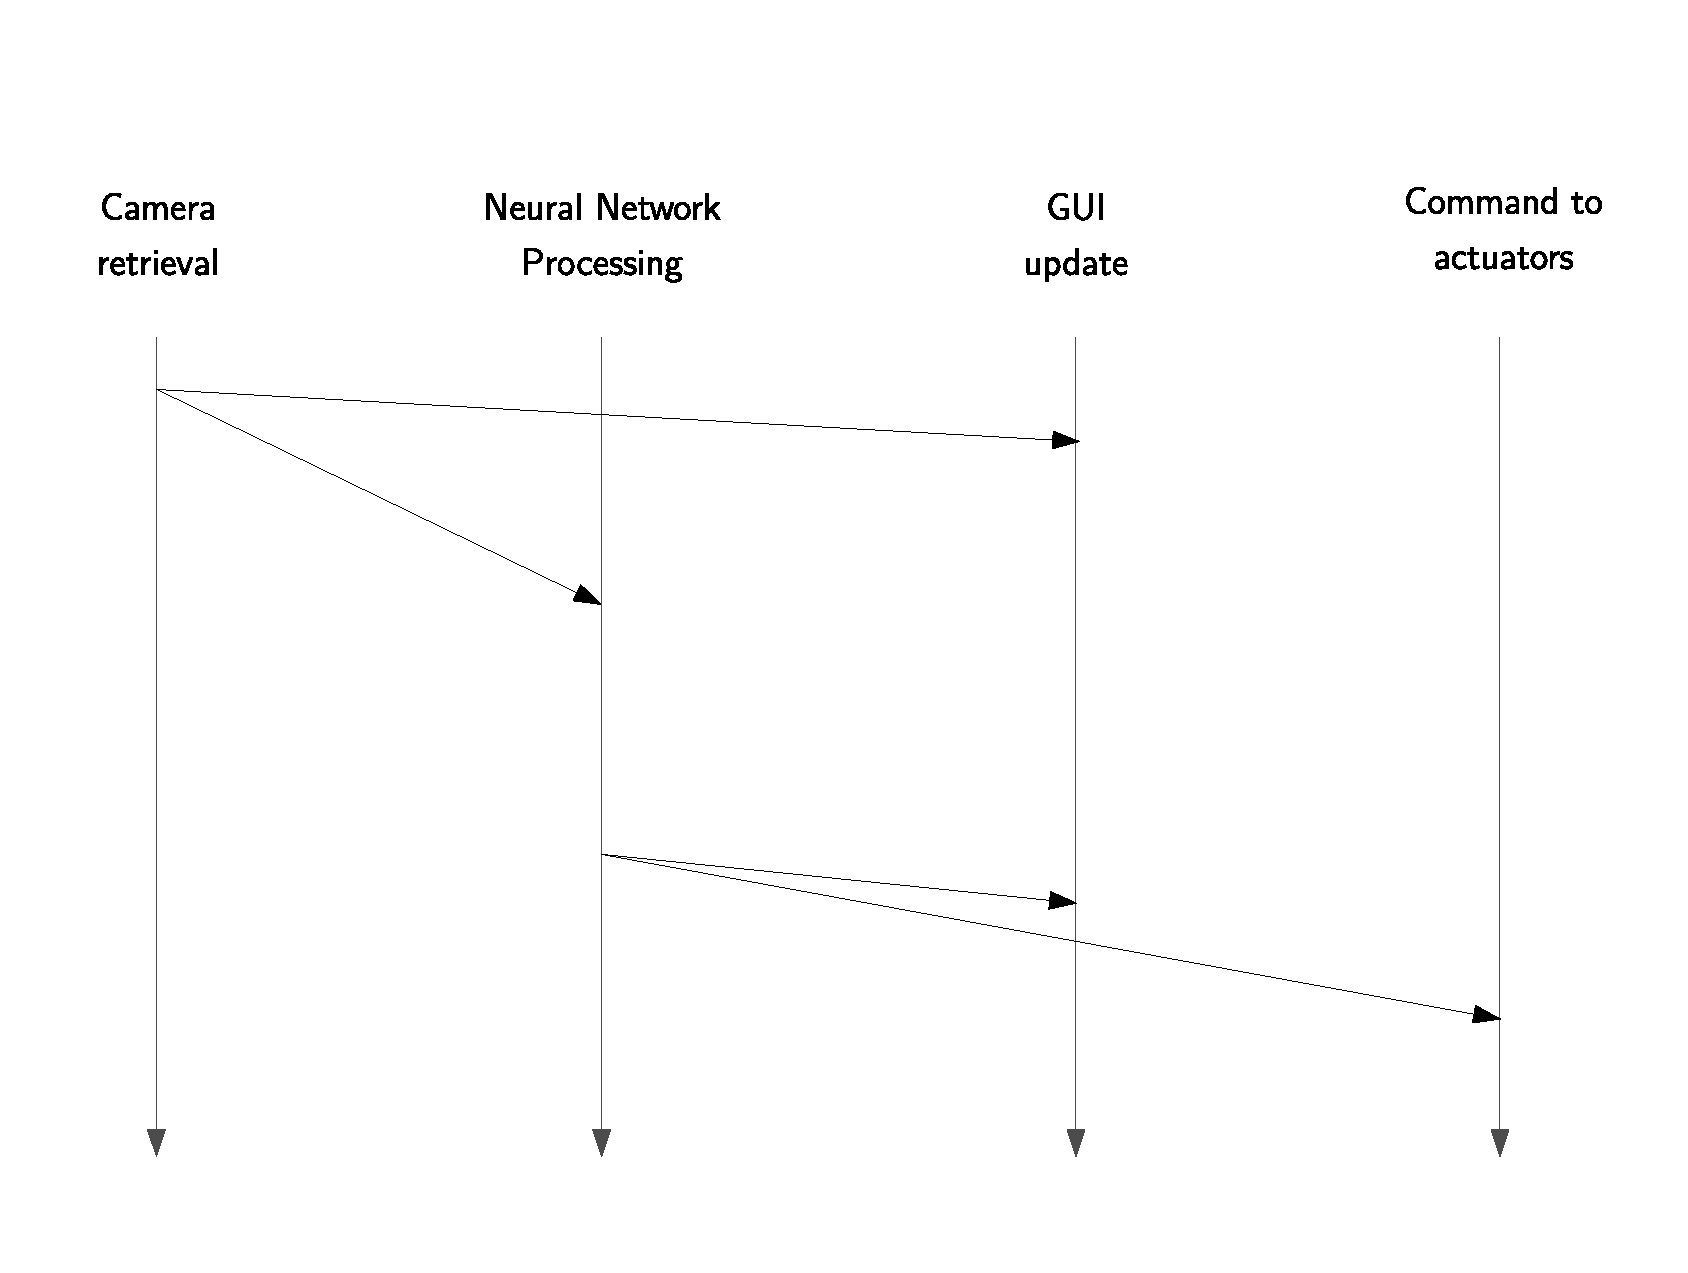
\includegraphics[width=3in]{images/tasks_threads}
		\caption{Parallel tasks to perform, and data exchange between them.}
		\label{fig:2_tasks}
	\end{figure}
	
	\item \textit{Implementation:} the next and most time consuming objective is to \textbf{develop both components}. The advantage is, once again, that both components are successive. This makes code reutilization a very interesting move, as we will only need to perform a language-friendly additions (on a simple way, thanks to \textit{Object Oriented Programming})) to the \texttt{Object Detector} code to implement the \texttt{Follow Person} features (depth images support, computing and commanding movements to the motors, among others). Details will be described on the appropriate section.
	
	\item \textit{Experimentation\footnote{\textit{"In theory, theory and practice are the same. In practice, they are not."}, Y. Berra}:} these nodes have a very strong tunability component (from neural network parameters to movement factors in the commands for the motors, stopping over describing all the desired behavior that the following algorithm has to adopt in several situations that it has to be capable of handling).
	
\end{itemize}

Finally, we will briefly highlight the \textbf{personal} objectives we have pursued on this project. As this has been developed along a whole year, and on a relatively abstract field as \emph{deep learning} is, a level of rigour has been necessary to accomplish satisfactory results. This provides a novice investigator the opportunity to learn about the phases and development process on a much more professional way than a homework task. \\

In addition, this project has allowed an interested person in \emph{deep learning} to learn about a cornucopia of concepts and experience. Later, when it was decided to evolve towards creating a reactive behavioral, it was motivating to make the most of a possible synergy between two different fields of knowledge, as \emph{deep learning} and \emph{robotics} are. It has to be remarked that the implementation of the development has always been possible, so it has been easy where there was more work to do in every moment.

\section{Methodology}
The workflow present on this project has been supported by weekly meetings.

MediaWiki

GitHub repo

Functional videos
